\documentclass[11pt,a4paper]{article}
\usepackage[utf8]{inputenc}
\usepackage[T1]{fontenc}
\usepackage{amsmath,amssymb,amsthm}
\usepackage{graphicx}
\usepackage{hyperref}
\usepackage{tikz}
\usepackage{algorithm}
\usepackage{algpseudocode}
\usepackage{booktabs}
\usepackage{geometry}
\usepackage{xcolor}

\geometry{margin=1in}
\usetikzlibrary{shapes,arrows,positioning,fit,backgrounds}

\title{\textbf{AZIMUTH: Adaptive Zero-shot Imitation via Multi-process Uncertainty-aware Transfer Hierarchy}}
\author{Process Control via Uncertainty-Aware Policy Optimization}
\date{\today}

\begin{document}

\maketitle

\begin{abstract}
Questo documento presenta l'architettura e il workflow del sistema AZIMUTH, un framework per l'ottimizzazione di catene di processi sequenziali in presenza di incertezza. Il sistema utilizza \textit{uncertainty predictors} per modellare la variabilità dei processi, \textit{policy generators} addestrabili per controllare gli input, e un \textit{surrogate model} per valutare la reliability delle trajectory generate. L'approccio sfrutta il \textit{sampling stocastico} per propagare l'incertezza attraverso l'intera catena di processi, permettendo al controller di apprendere politiche robuste in scenari non deterministici.
\end{abstract}

\tableofcontents
\newpage

\section{Introduzione}

\subsection{Motivazione}

Nei processi manifatturieri sequenziali (e.g., semiconduttori, stampa 3D, lavorazioni CNC), ogni processo produce output che diventano input per il processo successivo. Questi processi sono caratterizzati da:

\begin{itemize}
    \item \textbf{Incertezza intrinseca}: Anche con input identici, gli output variano
    \item \textbf{Dipendenze causali}: L'output del processo $i$ influenza il processo $i+1$
    \item \textbf{Adattività richiesta}: Il controller deve compensare errori accumulati
    \item \textbf{Obiettivi multipli}: Ogni processo ha target che dipendono dai risultati precedenti
\end{itemize}

\subsection{Obiettivo}

Dato:
\begin{itemize}
    \item Una sequenza di $N$ processi: $P_1 \to P_2 \to \cdots \to P_N$
    \item Una \textit{target trajectory} ottimale: $\{(a_i^*, o_i^*)\}_{i=1}^N$
    \item Un obiettivo di reliability target: $F^* \in [0,1]$
\end{itemize}

Trovare politiche $\{\pi_i\}_{i=1}^{N-1}$ che:
\begin{equation}
\pi_i: (o_{i-1}, \sigma_{i-1}^2, \text{scenario}) \mapsto a_i
\end{equation}

tali che la reliability della trajectory generata $F \approx F^*$ nonostante l'incertezza.

\section{Architettura del Sistema}

\subsection{Overview}

\begin{figure}[h]
\centering
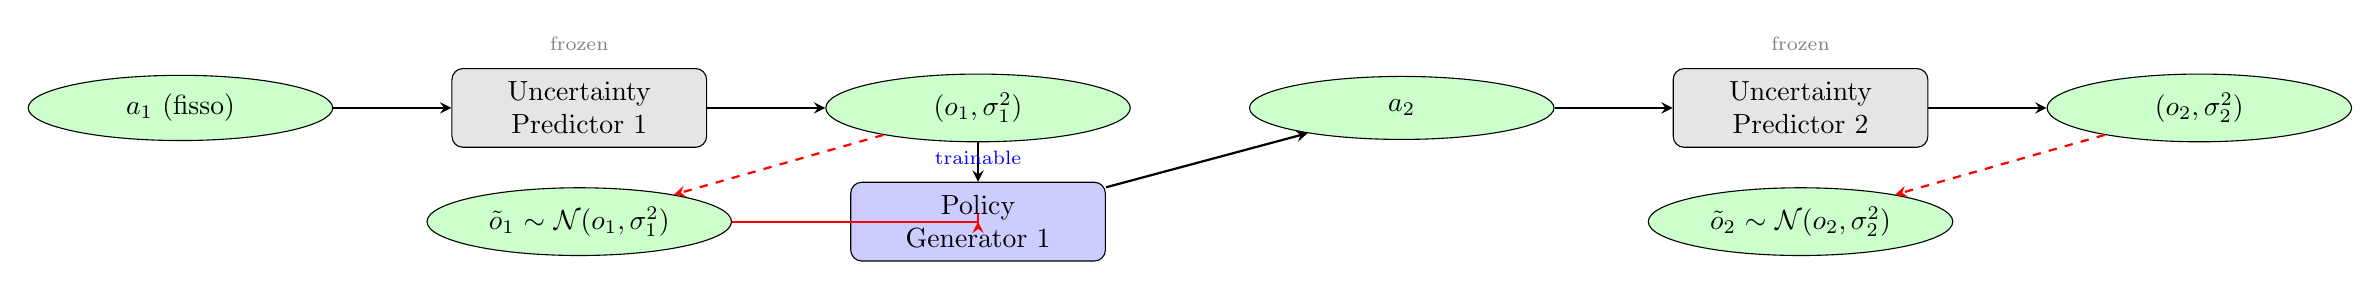
\begin{tikzpicture}[
    node distance=1.5cm,
    block/.style={rectangle, draw, fill=blue!20, text width=3cm, text centered, rounded corners, minimum height=1cm},
    frozen/.style={rectangle, draw, fill=gray!20, text width=3cm, text centered, rounded corners, minimum height=1cm},
    data/.style={ellipse, draw, fill=green!20, text width=2.5cm, text centered, minimum height=0.8cm},
    arrow/.style={->, >=stealth, thick}
]

% First process
\node[data] (a1) {$a_1$ (fisso)};
\node[frozen, right=of a1] (up1) {Uncertainty\\Predictor 1};
\node[data, right=of up1] (o1) {$(o_1, \sigma_1^2)$};

% Policy 1
\node[block, below=0.5cm of o1] (pol1) {Policy\\Generator 1};

% Second process
\node[data, right=of o1] (a2) {$a_2$};
\node[frozen, right=of a2] (up2) {Uncertainty\\Predictor 2};
\node[data, right=of up2] (o2) {$(o_2, \sigma_2^2)$};

% Arrows
\draw[arrow] (a1) -- (up1);
\draw[arrow] (up1) -- (o1);
\draw[arrow] (o1) -- (pol1);
\draw[arrow] (pol1) -- (a2);
\draw[arrow] (a2) -- (up2);
\draw[arrow] (up2) -- (o2);

% Sampling
\node[data, below=0.5cm of up1] (s1) {$\tilde{o}_1 \sim \mathcal{N}(o_1, \sigma_1^2)$};
\draw[arrow, dashed, red] (o1) -- (s1);
\draw[arrow, red] (s1) -| (pol1);

\node[data, below=0.5cm of up2] (s2) {$\tilde{o}_2 \sim \mathcal{N}(o_2, \sigma_2^2)$};
\draw[arrow, dashed, red] (o2) -- (s2);

% Labels
\node[above=0.1cm of up1, text=gray] {\scriptsize frozen};
\node[above=0.1cm of up2, text=gray] {\scriptsize frozen};
\node[above=0.1cm of pol1, text=blue] {\scriptsize trainable};

\end{tikzpicture}
\caption{Architettura della catena di processi. Gli \textit{Uncertainty Predictors} (frozen) predicono media e varianza, mentre i \textit{Policy Generators} (trainable) generano gli input per i processi successivi basandosi su output campionati stocasticamente.}
\label{fig:architecture}
\end{figure}

\subsection{Componenti Principali}

\subsubsection{Uncertainty Predictor}

Per ogni processo $P_i$, l'uncertainty predictor è una rete neurale $\mathcal{U}_i$ che predice:

\begin{equation}
\mathcal{U}_i(a_i) = (\mu_i, \sigma_i^2)
\end{equation}

dove:
\begin{itemize}
    \item $\mu_i \in \mathbb{R}^{d_i}$: output medio predetto
    \item $\sigma_i^2 \in \mathbb{R}^{d_i}$: varianza predetta (incertezza)
\end{itemize}

\textbf{Architettura}:
\begin{equation}
\begin{aligned}
h &= \text{ReLU}(W_h a_i + b_h) \\
\mu_i &= W_\mu h + b_\mu \\
\log(\sigma_i^2) &= W_\sigma h + b_\sigma \\
\sigma_i^2 &= \exp(\log(\sigma_i^2)) + \epsilon_{\min}
\end{aligned}
\end{equation}

dove $\epsilon_{\min} = 10^{-6}$ garantisce positività della varianza.

\textbf{Training}: Pre-addestrato su dati storici con loss:
\begin{equation}
\mathcal{L}_{\text{UP}} = \frac{1}{2}\log(2\pi\sigma_i^2) + \frac{(y_i - \mu_i)^2}{2\sigma_i^2}
\end{equation}

\textbf{Status}: \textcolor{red}{Frozen durante l'ottimizzazione del controller}.

\subsubsection{Sampling Stocastico}

Dopo la predizione di $(\mu_i, \sigma_i^2)$, l'output effettivo viene campionato usando il \textbf{reparameterization trick}:

\begin{equation}
\boxed{\tilde{o}_i = \mu_i + \epsilon \odot \sigma_i \quad \text{con} \quad \epsilon \sim \mathcal{N}(0, I)}
\end{equation}

\textbf{Proprietà chiave}:
\begin{itemize}
    \item \textbf{Differenziabilità}: I gradienti fluiscono attraverso $\mu_i$ e $\sigma_i$
    \item \textbf{Stocasticità}: Ogni forward pass genera output diversi
    \item \textbf{Realismo}: Simula la variabilità intrinseca dei processi
\end{itemize}

\subsubsection{Policy Generator}

Per $i = 1, \ldots, N-1$, il policy generator $\pi_i$ è una rete neurale trainable che genera gli input per il processo successivo:

\begin{equation}
a_{i+1} = \pi_i(\tilde{o}_i, \sigma_i^2, e_{\text{scenario}})
\end{equation}

dove:
\begin{itemize}
    \item $\tilde{o}_i$: output campionato del processo precedente
    \item $\sigma_i^2$: incertezza predetta
    \item $e_{\text{scenario}}$: embedding dello scenario (parametri strutturali)
\end{itemize}

\textbf{Architettura}:
\begin{equation}
\begin{aligned}
x &= [\tilde{o}_i; \sigma_i^2; e_{\text{scenario}}] \\
h_1 &= \text{ReLU}(W_1 x + b_1) \\
h_2 &= \text{ReLU}(W_2 h_1 + b_2) \\
a_{i+1} &= W_3 h_2 + b_3
\end{aligned}
\end{equation}

\subsubsection{Scenario Encoder}

Alcuni parametri di input sono \textit{non controllabili} (e.g., temperatura ambiente, proprietà del materiale). Il \textit{scenario encoder} mappa questi parametri strutturali in un embedding:

\begin{equation}
e_{\text{scenario}} = \text{ScenarioEncoder}(p_{\text{structural}})
\end{equation}

Questo permette al policy generator di adattarsi a diversi contesti operativi.

\section{Forward Pass: ProcessChain}

\subsection{Algoritmo}

\begin{algorithm}[H]
\caption{ProcessChain Forward Pass}
\begin{algorithmic}[1]
\State \textbf{Input:} $a_1^*$ (input iniziale fisso), scenario index $s$
\State \textbf{Output:} Trajectory $\mathcal{T} = \{(a_i, \mu_i, \sigma_i^2, \tilde{o}_i)\}_{i=1}^N$

\State $e_s \gets \text{ScenarioEncoder}(p_{\text{structural}}^{(s)})$
\State $a_1 \gets a_1^*$ \Comment{Input iniziale fisso}

\For{$i = 1$ \textbf{to} $N$}
    \State \textcolor{gray}{// 1. Predizione con uncertainty}
    \State $a_i^{\text{scaled}} \gets \text{InputScaler}_i(a_i)$
    \State $(\mu_i^{\text{scaled}}, \sigma_i^{2,\text{scaled}}) \gets \mathcal{U}_i(a_i^{\text{scaled}})$ \Comment{Frozen}
    \State $\mu_i \gets \text{OutputScaler}_i^{-1}(\mu_i^{\text{scaled}})$
    \State $\sigma_i^2 \gets \text{UnscaleVariance}_i(\sigma_i^{2,\text{scaled}})$

    \State \textcolor{gray}{// 2. Sampling stocastico}
    \State $\epsilon \sim \mathcal{N}(0, I)$
    \State $\tilde{o}_i \gets \mu_i + \epsilon \odot \sqrt{\sigma_i^2 + 10^{-8}}$ \Comment{\textcolor{red}{Reparameterization}}

    \State \textcolor{gray}{// 3. Store in trajectory}
    \State $\mathcal{T}[P_i] \gets \{a_i, \mu_i, \sigma_i^2, \tilde{o}_i\}$

    \If{$i < N$}
        \State \textcolor{gray}{// 4. Policy genera prossimo input}
        \State $x \gets [\tilde{o}_i; \sigma_i^2; e_s]$ \Comment{\textcolor{red}{Usa output campionato}}
        \State $a_{i+1}^{\text{gen}} \gets \pi_i(x)$ \Comment{Trainable}
        \State $a_{i+1} \gets \text{ApplyConstraints}(a_{i+1}^{\text{gen}}, s)$ \Comment{Fissa parametri non-controllabili}
    \EndIf
\EndFor

\State \Return $\mathcal{T}$
\end{algorithmic}
\end{algorithm}

\subsection{Propagazione dell'Incertezza}

Un aspetto cruciale è che il policy generator $\pi_i$ riceve come input \textbf{l'output campionato} $\tilde{o}_i$, non la media $\mu_i$. Questo significa:

\begin{equation}
a_{i+1} = \pi_i(\tilde{o}_i, \sigma_i^2, e_s) \quad \text{\textcolor{red}{← Stocastico!}}
\end{equation}

\textbf{Conseguenze}:
\begin{enumerate}
    \item \textbf{Propagazione}: Errori nei processi iniziali si propagano
    \item \textbf{Robustezza}: Il controller deve imparare a compensare variazioni
    \item \textbf{Realismo}: Simula feedback non deterministico del mondo reale
\end{enumerate}

\section{Reliability Computation: Surrogate Model}

\subsection{Obiettivo}

Il \textit{surrogate model} (ProT) valuta la qualità complessiva di una trajectory:

\begin{equation}
F = \text{ProT}(\mathcal{T}) \in [0, 1]
\end{equation}

dove $F = 1$ indica una trajectory perfetta e $F = 0$ indica fallimento completo.

\subsection{Adaptive Targets}

Ogni processo ha un \textit{target adattivo} che dipende dagli output dei processi precedenti. Questo modella le dipendenze causali:

\subsubsection{Esempio: Sistema a 4 Processi}

\textbf{1. LASER} (primo processo, target fisso):
\begin{equation}
\begin{aligned}
\tau_{\text{laser}} &= 0.5 \quad \text{(fisso)} \\
q_{\text{laser}} &= \exp\left(-\frac{(\tilde{o}_{\text{laser}} - 0.5)^2}{0.1}\right)
\end{aligned}
\end{equation}

\textbf{2. PLASMA} (target dipende da Laser):
\begin{equation}
\begin{aligned}
\tau_{\text{plasma}} &= 5.0 + 20.0 \cdot (\tilde{o}_{\text{laser}} - 0.5) \\
q_{\text{plasma}} &= \exp\left(-\frac{(\tilde{o}_{\text{plasma}} - \tau_{\text{plasma}})^2}{2.0}\right)
\end{aligned}
\end{equation}

\textit{Interpretazione}: Se il laser è troppo forte ($\tilde{o}_{\text{laser}} > 0.5$), il plasma deve aumentare il removal rate per compensare.

\textbf{3. GALVANIC} (target dipende da Laser e Plasma):
\begin{equation}
\begin{aligned}
\tau_{\text{galvanic}} &= 10.0 + 5.0 \cdot (\tilde{o}_{\text{plasma}} - 5.0) + 4.0 \cdot (\tilde{o}_{\text{laser}} - 0.5) \\
q_{\text{galvanic}} &= \exp\left(-\frac{(\tilde{o}_{\text{galvanic}} - \tau_{\text{galvanic}})^2}{4.0}\right)
\end{aligned}
\end{equation}

\textbf{4. MICROETCH} (target dipende da tutti i precedenti):
\begin{equation}
\begin{aligned}
\tau_{\text{microetch}} &= 20.0 + 15.0 \cdot (\tilde{o}_{\text{laser}} - 0.5) \\
&\quad + 3.0 \cdot (\tilde{o}_{\text{plasma}} - 5.0) \\
&\quad - 1.5 \cdot (\tilde{o}_{\text{galvanic}} - 10.0) \\
q_{\text{microetch}} &= \exp\left(-\frac{(\tilde{o}_{\text{microetch}} - \tau_{\text{microetch}})^2}{4.0}\right)
\end{aligned}
\end{equation}

\subsection{Reliability Aggregation}

La reliability finale è una media pesata delle qualità individuali:

\begin{equation}
F = \frac{\sum_{i=1}^N w_i \cdot q_i}{\sum_{i=1}^N w_i}
\end{equation}

dove i pesi $w_i$ riflettono l'importanza relativa di ogni processo (e.g., $w_{\text{galvanic}} = 0.5$, gli altri $0.15-0.2$).

\subsection{Uso degli Output Campionati}

Crucialmente, il calcolo di reliability usa gli \textbf{output già campionati}:

\begin{equation}
F = \text{ProT}(\{\tilde{o}_i\}_{i=1}^N)
\end{equation}

Questo significa che:
\begin{itemize}
    \item $F$ è stocastico (varia ad ogni forward pass)
    \item Il controller impara a massimizzare $\mathbb{E}[F]$ nonostante la variabilità
    \item I gradienti fluiscono attraverso il sampling
\end{itemize}

\section{Training: Controller Optimization}

\subsection{Loss Function}

Il controller viene addestrato per minimizzare:

\begin{equation}
\boxed{\mathcal{L}_{\text{total}} = \alpha \cdot \mathcal{L}_{\text{reliability}} + \lambda_{\text{BC}} \cdot \mathcal{L}_{\text{BC}}}
\end{equation}

\subsubsection{Reliability Loss}

Misura la distanza dalla reliability target:

\begin{equation}
\mathcal{L}_{\text{reliability}} = \frac{1}{B} \sum_{s=1}^B (F_s - F_s^*)^2
\end{equation}

dove:
\begin{itemize}
    \item $B$: batch size (numero di scenari)
    \item $F_s$: reliability della trajectory generata per scenario $s$
    \item $F_s^*$: reliability target per scenario $s$ (calcolata su target trajectory)
\end{itemize}

\textbf{Scaling}: Il coefficiente $\alpha$ bilancia l'importanza di questa loss. Tipicamente $\alpha = 100$ per dare peso significativo alla reliability.

\subsubsection{Behavioral Cloning Loss}

Regolarizza il policy generator per rimanere vicino agli input target:

\begin{equation}
\mathcal{L}_{\text{BC}} = \frac{1}{B \cdot N} \sum_{s=1}^B \sum_{i=2}^N \|a_i^{(s)} - a_i^{*,(s)}\|_2^2
\end{equation}

\textbf{Rationale}:
\begin{itemize}
    \item Previene soluzioni patologiche
    \item Fornisce un "punto di partenza" sensato
    \item Riduce l'esplorazione necessaria
\end{itemize}

\textbf{Weight}: Tipicamente $\lambda_{\text{BC}} = 0.1$ (meno importante della reliability).

\subsection{Training Algorithm}

\begin{algorithm}[H]
\caption{Controller Training Loop}
\begin{algorithmic}[1]
\State \textbf{Input:} Target trajectory $\mathcal{T}^*$, num epochs $E$, batch size $B$
\State Initialize policy generators $\{\pi_i\}_{i=1}^{N-1}$
\State Load frozen uncertainty predictors $\{\mathcal{U}_i\}_{i=1}^N$
\State Compute $F^* = \text{ProT}(\mathcal{T}^*)$ for all scenarios

\For{epoch $= 1$ \textbf{to} $E$}
    \State Sample batch of scenarios: $\mathcal{S} = \{s_1, \ldots, s_B\}$

    \For{$s \in \mathcal{S}$}
        \State \textcolor{gray}{// Forward pass (Algorithm 1)}
        \State $\mathcal{T}_s \gets \text{ProcessChain.forward}(\text{scenario}=s)$

        \State \textcolor{gray}{// Compute reliability}
        \State $F_s \gets \text{ProT}(\mathcal{T}_s)$ \Comment{Usa $\tilde{o}_i$ campionati}
    \EndFor

    \State \textcolor{gray}{// Compute losses}
    \State $\mathcal{L}_{\text{rel}} \gets \frac{1}{B} \sum_{s \in \mathcal{S}} (F_s - F_s^*)^2$
    \State $\mathcal{L}_{\text{BC}} \gets \frac{1}{B \cdot N} \sum_{s \in \mathcal{S}} \sum_{i=2}^N \|a_i^{(s)} - a_i^{*,(s)}\|_2^2$
    \State $\mathcal{L}_{\text{total}} \gets \alpha \cdot \mathcal{L}_{\text{rel}} + \lambda_{\text{BC}} \cdot \mathcal{L}_{\text{BC}}$

    \State \textcolor{gray}{// Backpropagation}
    \State $\mathcal{L}_{\text{total}}.\text{backward}()$
    \State Update $\{\pi_i\}$ with optimizer (e.g., Adam)

    \If{epoch mod 100 == 0}
        \State Log metrics: $F$, $F^*$, losses
    \EndIf
\EndFor
\end{algorithmic}
\end{algorithm}

\subsection{Gradient Flow}

Il gradiente fluisce attraverso:

\begin{equation}
\frac{\partial \mathcal{L}}{\partial \theta_{\pi_i}} = \frac{\partial \mathcal{L}}{\partial F} \cdot \frac{\partial F}{\partial \tilde{o}_j} \cdot \frac{\partial \tilde{o}_j}{\partial \mu_j} \cdot \frac{\partial \mu_j}{\partial a_j} \cdot \frac{\partial a_j}{\partial \theta_{\pi_i}}
\end{equation}

dove:
\begin{itemize}
    \item $\frac{\partial F}{\partial \tilde{o}_j}$: Sensibilità della reliability agli output
    \item $\frac{\partial \tilde{o}_j}{\partial \mu_j} = 1$ (reparameterization trick)
    \item $\frac{\partial \mu_j}{\partial a_j}$: Frozen (attraversa uncertainty predictor)
    \item $\frac{\partial a_j}{\partial \theta_{\pi_i}}$: Policy gradient
\end{itemize}

\section{Multi-Scenario Training}

\subsection{Motivazione}

Il controller deve funzionare in \textit{condizioni diverse}:
\begin{itemize}
    \item Diverse temperature ambientali
    \item Diversi lotti di materiale
    \item Diverse condizioni iniziali
\end{itemize}

\subsection{Scenario Encoding}

Ogni scenario $s$ è caratterizzato da:
\begin{equation}
p_{\text{structural}}^{(s)} = [\text{Temp}_{\text{ambient}}, \text{Material}_{\text{prop}}, \ldots]
\end{equation}

Questi parametri vengono codificati in un embedding:

\begin{equation}
e_s = \text{ScenarioEncoder}(p_{\text{structural}}^{(s)})
\end{equation}

e concatenati con gli output per condizionare il policy generator:

\begin{equation}
a_{i+1} = \pi_i([\tilde{o}_i; \sigma_i^2; e_s])
\end{equation}

\subsection{Scenario-Specific $F^*$}

Ogni scenario ha un suo target reliability:

\begin{equation}
F_s^* = \text{ProT}(\mathcal{T}^*_s)
\end{equation}

dove $\mathcal{T}^*_s$ è la target trajectory per scenario $s$.

\textbf{Nota}: Per calcolare $F^*$, si usa $\sigma^2 = 0$ (nessuna incertezza), quindi:

\begin{equation}
F_s^* = \text{ProT}(\{o_i^{*,(s)}\}_{i=1}^N) \quad \text{\textcolor{blue}{← Deterministico}}
\end{equation}

\section{Stocasticità vs Determinismo}

\subsection{Durante Training}

\textbf{Actual Trajectory} (generata dal controller):
\begin{itemize}
    \item ✓ Sampling stocastico: $\tilde{o}_i \sim \mathcal{N}(\mu_i, \sigma_i^2)$
    \item ✓ Ogni epoch vede realizzazioni diverse
    \item ✓ Il controller impara robustezza
\end{itemize}

\textbf{Target Trajectory} (calcolo di $F^*$):
\begin{itemize}
    \item ✗ NO sampling: usa $o_i^*$ direttamente
    \item ✓ $F^*$ è un target fisso
    \item ✓ Facilita la convergenza
\end{itemize}

\subsection{Vantaggi del Sampling Stocastico}

\begin{enumerate}
    \item \textbf{Realismo}: Simula variabilità intrinseca dei processi
    \item \textbf{Robustezza}: Controller impara a gestire incertezza
    \item \textbf{Esplorazione implicita}: Vede diverse realizzazioni ogni epoch
    \item \textbf{Gradient informativeness}: Varianza negli output guida l'ottimizzazione
\end{enumerate}

\subsection{Confronto}

\begin{table}[h]
\centering
\begin{tabular}{lcc}
\toprule
\textbf{Aspetto} & \textbf{Deterministico} & \textbf{Stocastico} \\
\midrule
Output & $o_i = \mu_i$ & $\tilde{o}_i = \mu_i + \epsilon \sigma_i$ \\
Reliability & $F$ fisso per input fisso & $F$ varia ogni run \\
Gradienti & Stabili & Più variabili \\
Convergenza & Più veloce & Potenzialmente più lenta \\
Robustezza finale & Minore & \textbf{Maggiore} \\
Realismo & Limitato & \textbf{Alto} \\
\bottomrule
\end{tabular}
\caption{Confronto tra approccio deterministico e stocastico}
\end{table}

\section{Considerazioni Implementative}

\subsection{Scaling}

Gli uncertainty predictors lavorano in spazio normalizzato:

\begin{equation}
\begin{aligned}
a_i^{\text{scaled}} &= \frac{a_i - \mu_{a_i}}{\sigma_{a_i}} \\
\mu_i^{\text{orig}} &= \mu_i^{\text{scaled}} \cdot \sigma_{o_i} + \mu_{o_i} \\
\sigma_i^{2,\text{orig}} &= \sigma_i^{2,\text{scaled}} \cdot \sigma_{o_i}^2
\end{aligned}
\end{equation}

\subsection{Numerical Stability}

Per evitare problemi numerici:
\begin{equation}
\sigma_i^2 = \exp(\log(\sigma_i^2)) + 10^{-6}
\end{equation}

Per il sampling:
\begin{equation}
\tilde{o}_i = \mu_i + \epsilon \odot \sqrt{\sigma_i^2 + 10^{-8}}
\end{equation}

\subsection{Hyperparameters}

\begin{table}[h]
\centering
\begin{tabular}{ll}
\toprule
\textbf{Parametro} & \textbf{Valore tipico} \\
\midrule
Learning rate & $10^{-3}$ - $10^{-4}$ \\
Batch size & 4-8 scenari \\
Reliability weight $\alpha$ & 100 \\
BC weight $\lambda_{\text{BC}}$ & 0.1 \\
Optimizer & Adam \\
Epochs & 5000-10000 \\
Policy hidden sizes & [64, 32] \\
Scenario embedding dim & 16 \\
\bottomrule
\end{tabular}
\caption{Hyperparameters tipici}
\end{table}

\section{Workflow Completo: Schema Riassuntivo}

\begin{figure}[h]
\centering
\begin{tikzpicture}[
    node distance=1cm,
    phase/.style={rectangle, draw, fill=orange!20, text width=4cm, text centered, rounded corners, minimum height=1cm, font=\small},
    step/.style={rectangle, draw, fill=blue!15, text width=4.5cm, align=left, minimum height=0.8cm, font=\scriptsize},
    arrow/.style={->, >=stealth, thick}
]

% Phases
\node[phase] (phase1) {\textbf{1. Pre-Training}};
\node[phase, below=0.3cm of phase1] (phase2) {\textbf{2. Controller Initialization}};
\node[phase, below=0.3cm of phase2] (phase3) {\textbf{3. Training Loop}};
\node[phase, below=0.3cm of phase3] (phase4) {\textbf{4. Inference}};

% Steps for Phase 1
\node[step, right=0.5cm of phase1] (s1a) {Train uncertainty predictors su dati storici};
\node[step, below=0.1cm of s1a] (s1b) {Freeze: no più update};

% Steps for Phase 2
\node[step, right=0.5cm of phase2] (s2a) {Initialize policy generators};
\node[step, below=0.1cm of s2a] (s2b) {Create scenario encoder};
\node[step, below=0.1cm of s2b] (s2c) {Generate target trajectory $\mathcal{T}^*$};
\node[step, below=0.1cm of s2c] (s2d) {Compute $F^*$ per ogni scenario};

% Steps for Phase 3
\node[step, right=0.5cm of phase3] (s3a) {Sample batch di scenari};
\node[step, below=0.1cm of s3a] (s3b) {Forward: genera trajectory con sampling};
\node[step, below=0.1cm of s3b] (s3c) {Compute $F$ su output campionati};
\node[step, below=0.1cm of s3c] (s3d) {Loss: $(F-F^*)^2 + \text{BC}$};
\node[step, below=0.1cm of s3d] (s3e) {Backprop + update policies};

% Steps for Phase 4
\node[step, right=0.5cm of phase4] (s4a) {Input: scenario + $a_1$};
\node[step, below=0.1cm of s4a] (s4b) {Forward: genera trajectory};
\node[step, below=0.1cm of s4b] (s4c) {Output: $(a_i, \tilde{o}_i, F)$};

% Arrows
\draw[arrow] (phase1) -- (phase2);
\draw[arrow] (phase2) -- (phase3);
\draw[arrow] (phase3) -- (phase4);

\end{tikzpicture}
\caption{Workflow completo del sistema AZIMUTH}
\end{figure}

\section{Esempio Concreto}

Consideriamo un sistema semplificato a 2 processi: LASER → PLASMA.

\subsection{Setup}

\textbf{Processo 1 (LASER)}:
\begin{itemize}
    \item Input: $a_1 = [\text{PowerTarget}, \text{Temp}_{\text{ambient}}]$
    \item Output: $o_1 = \text{ActualPower}$
\end{itemize}

\textbf{Processo 2 (PLASMA)}:
\begin{itemize}
    \item Input: $a_2 = [\text{RF\_Power}, \text{Duration}]$
    \item Output: $o_2 = \text{RemovalRate}$
\end{itemize}

\textbf{Target trajectory}:
\begin{equation}
\mathcal{T}^* = \{(a_1^* = [0.5, 25], o_1^* = 0.48), (a_2^* = [200, 30], o_2^* = 5.2)\}
\end{equation}

\subsection{Training Step}

\textbf{1. Forward Pass}:

\begin{align}
a_1 &= [0.5, 25] \quad \text{(fisso)} \\
(\mu_1, \sigma_1^2) &= \mathcal{U}_1(a_1) = (0.48, 0.01) \\
\tilde{o}_1 &= 0.48 + \epsilon \cdot \sqrt{0.01} \approx 0.46 \quad \text{(campionato)} \\
a_2 &= \pi_1([\tilde{o}_1, \sigma_1^2, e_s]) = [195, 32] \quad \text{(generato)} \\
(\mu_2, \sigma_2^2) &= \mathcal{U}_2(a_2) = (4.8, 0.05) \\
\tilde{o}_2 &= 4.8 + \epsilon \cdot \sqrt{0.05} \approx 4.95 \quad \text{(campionato)}
\end{align}

\textbf{2. Reliability Computation}:

\begin{align}
\tau_{\text{laser}} &= 0.5 \\
q_{\text{laser}} &= \exp(-(\tilde{o}_1 - 0.5)^2 / 0.1) = \exp(-0.16) \approx 0.85 \\
\tau_{\text{plasma}} &= 5.0 + 20 \cdot (\tilde{o}_1 - 0.5) = 5.0 - 0.8 = 4.2 \\
q_{\text{plasma}} &= \exp(-(\tilde{o}_2 - 4.2)^2 / 2.0) = \exp(-0.28) \approx 0.76 \\
F &= \frac{0.2 \cdot 0.85 + 0.15 \cdot 0.76}{0.2 + 0.15} \approx 0.81
\end{align}

\textbf{3. Loss Computation}:

\begin{align}
F^* &= 0.95 \quad \text{(calcolato su } \mathcal{T}^*) \\
\mathcal{L}_{\text{rel}} &= (0.81 - 0.95)^2 = 0.0196 \\
\mathcal{L}_{\text{BC}} &= \|[195,32] - [200,30]\|^2 = 29 \\
\mathcal{L}_{\text{total}} &= 100 \cdot 0.0196 + 0.1 \cdot 29 = 1.96 + 2.9 = 4.86
\end{align}

\textbf{4. Gradient Update}:

Il gradiente $\nabla_{\theta_{\pi_1}} \mathcal{L}_{\text{total}}$ guida $\pi_1$ a generare $a_2$ che aumenti $F$. Tipicamente:
\begin{itemize}
    \item $\tilde{o}_1 < \tau_{\text{laser}}$ ⇒ aumenta $a_2$ per compensare
    \item $\sigma_1^2$ alta ⇒ strategie più conservative
\end{itemize}

\section{Conclusioni}

\subsection{Contributi Principali}

\begin{enumerate}
    \item \textbf{Uncertainty-aware control}: Predittori di incertezza forniscono sia media che varianza
    \item \textbf{Stochastic sampling}: Output campionati rendono il sistema realistico
    \item \textbf{Propagazione dell'incertezza}: Feedback stocastico attraverso la catena
    \item \textbf{Adaptive reliability}: Target che si adattano ai processi precedenti
    \item \textbf{Multi-scenario training}: Generalizzazione a diverse condizioni
\end{enumerate}

\subsection{Vantaggi}

\begin{itemize}
    \item \textbf{Robustezza}: Controller impara a gestire variabilità
    \item \textbf{Modularità}: Processi indipendenti collegati da policies
    \item \textbf{Scalabilità}: Facilmente estendibile a $N$ processi
    \item \textbf{Interpretabilità}: Componenti con ruoli chiari
\end{itemize}

\subsection{Limitazioni}

\begin{itemize}
    \item Richiede uncertainty predictors pre-addestrati
    \item Gradienti stocastici possono rallentare convergenza
    \item Surrogate model (ProT) è ancora semplificato
    \item Assume Gaussianità delle distribuzioni
\end{itemize}

\subsection{Direzioni Future}

\begin{enumerate}
    \item Sostituire ProT placeholder con vero transformer
    \item Esplorare distribuzioni non-Gaussiane (e.g., mixture models)
    \item Aggiungere constraints fisici hard (e.g., safety limits)
    \item Online adaptation: fine-tuning durante deployment
    \item Multi-objective optimization: bilanciare reliability, costo, throughput
\end{enumerate}

\appendix

\section{Notazione}

\begin{table}[h]
\centering
\begin{tabular}{ll}
\toprule
\textbf{Simbolo} & \textbf{Significato} \\
\midrule
$N$ & Numero di processi nella catena \\
$P_i$ & Processo $i$-esimo \\
$a_i$ & Input al processo $i$ \\
$o_i$ & Output del processo $i$ \\
$\mu_i$ & Media predetta per output processo $i$ \\
$\sigma_i^2$ & Varianza predetta per output processo $i$ \\
$\tilde{o}_i$ & Output campionato: $\tilde{o}_i \sim \mathcal{N}(\mu_i, \sigma_i^2)$ \\
$\mathcal{U}_i$ & Uncertainty predictor per processo $i$ (frozen) \\
$\pi_i$ & Policy generator $i$: genera $a_{i+1}$ (trainable) \\
$e_s$ & Embedding dello scenario $s$ \\
$\mathcal{T}$ & Trajectory: $\{(a_i, \mu_i, \sigma_i^2, \tilde{o}_i)\}_{i=1}^N$ \\
$\mathcal{T}^*$ & Target trajectory (ottimale) \\
$F$ & Reliability della trajectory generata \\
$F^*$ & Reliability target \\
$\tau_i$ & Target adattivo per processo $i$ \\
$q_i$ & Quality score per processo $i$ \\
$w_i$ & Peso relativo del processo $i$ \\
$\alpha$ & Coefficiente per reliability loss \\
$\lambda_{\text{BC}}$ & Coefficiente per behavioral cloning loss \\
\bottomrule
\end{tabular}
\end{table}

\section{Codice di Riferimento}

File principali:
\begin{itemize}
    \item \texttt{controller\_optimization/src/utils/process\_chain.py}: ProcessChain
    \item \texttt{controller\_optimization/src/models/surrogate.py}: ProTSurrogate
    \item \texttt{controller\_optimization/src/models/policy\_generator.py}: Policy
    \item \texttt{controller\_optimization/src/models/scenario\_encoder.py}: Encoder
    \item \texttt{uncertainty\_predictor/src/models/uncertainty\_nn.py}: $\mathcal{U}_i$
\end{itemize}

\end{document}
